%
% File acl2014.tex
%
% Contact: g.colavizza@uva.nl
%%
%% Based on the style files for ACL-2013, which were, in turn,
%% Based on the style files for ACL-2012, which were, in turn,
%% based on the style files for ACL-2011, which were, in turn, 
%% based on the style files for ACL-2010, which were, in turn, 
%% based on the style files for ACL-IJCNLP-2009, which were, in turn,
%% based on the style files for EACL-2009 and IJCNLP-2008...

%% Based on the style files for EACL 2006 by 
%%e.agirre@ehu.es or Sergi.Balari@uab.es
%% and that of ACL 08 by Joakim Nivre and Noah Smith

\documentclass[11pt]{article}
\usepackage{acl2014}
\usepackage{times}
\usepackage{url}
\usepackage{latexsym}
\usepackage{graphicx}
\usepackage{float} 

%\setlength\titlebox{5cm}

% You can expand the titlebox if you need extra space
% to show all the authors. Please do not make the titlebox
% smaller than 5cm (the original size); we will check this
% in the camera-ready version and ask you to change it back.


\title{Voci dal braccio della morte: un'indagine tra linguaggio ed emozioni}

\author{Erica Solinas \\
  {\tt erica.solinas@studio.unibo.it} 
}
\date{}

\begin{document}
\maketitle
\begin{abstract}
  Questo progetto si propone di creare un dataset completo che raccolga informazioni personali, riassunti dei reati e ultime dichiarazioni dei 591 condannati a morte giustiziati in Texas dal 1982 al 2024. Tramite tecniche di web scraping e OCR, i dati sono stati estratti, strutturati e analizzati con un focus sulle emozioni espresse nelle ultime parole dei condannati, la cui analisi è stata effettuata attraverso le API di OpenAI.

\end{abstract}

\section{Introduzione}

Il progetto è stato concepito con l’obiettivo di applicare le tecnologie studiate durante il corso, esplorando al contempo anche ulteriori strumenti e tecniche necessari alla sua realizzazione. Ciò ci ha permesso di sviluppare una comprensione generale delle diverse soluzioni disponibili, ampliando le competenze acquisite, seppur in modo sommario.

Abbiamo scelto di concentrarci sulla realizzazione di un progetto di natura linguistica e, fin dall'inizio, abbiamo mostrato un forte interesse per il sito del TDCJ (\textit{Texas Department of Criminal Justice}). Abbiamo voluto ascoltare le loro voci, far emergere i loro sentimenti più profondi, leggere le ragioni dietro la loro condanna e scoprire se, nei loro ultimi istanti di vita, confessavano la loro colpa o cercavano di affermare la propria innocenza. 

A tale scopo, abbiamo dovuto creare il dataset da cui partire attraverso il web scraping dell'intero sito\footnote{\url{https://www.tdcj.texas.gov/death_row/dr_executed_offenders.html}}, al fine di creare un file CSV che riproducesse una tabella simile su cui poter effettuare tutte le opportune analisi. A questo punto abbiamo deciso di realizzare due tipi di analisi: una sui dati demografici dei condannati e una lessicale sui riassunti delle loro cause di condanna e sulle loro ultime dichiarazioni. Quest'ultime sono state il focus centrale della fase successiva, in cui abbiamo usato le API di OpenAI per estrarne i sentimenti espressi e per riconoscere se in quelle parole l'imputato si dichiava colpevole, innocente o non lo specificava. Nell'ultima fase abbiamo preso un campione del nostro dataset e l'abbiamo annotato manualmente per valutare le performance del modello. 

\section{Fase 1: Web Scraping}
Per la fase di Web Scraping sono state utilizzate librerie fondamentali come {\tt BeautifulSoup}, {\tt requests} e {\tt urllib}. L’obiettivo principale era la creazione di un dataset strutturato in un file CSV contenente tutte le informazioni sui detenuti presenti sul sito del TDCJ. Questa fase si è rivelata particolarmente lunga e complessa a causa di alcune problematiche legate alla struttura HTML del sito. In particolare, è stato necessario implementare una funzione specifica per gestire due link dei condannati, poiché la loro struttura differiva dal resto della pagina HTML. Inoltre, alcune informazioni chiave, come i riassunti delle cause di condanna (\textit{“Summary of Incident”}) e il livello di istruzione (\textit{“Education Level”}), erano presenti nella sezione “Inmate Information” del sito, ma in tanti casi erano salvate come immagini in formato {\tt .jpg} anziché testo. Per ovviare a questo problema, è stato utilizzato un OCR ({\tt easyocr}) per estrarre il testo dalle immagini, affiancato dalle API di OpenAI per migliorare la qualità dei dati estratti. Tuttavia, l’OCR non ha sempre restituito risultati ottimali, generando alcune imprecisioni che hanno introdotto del rumore nel dataset finale. Nonostante queste difficoltà, i dati sono stati integrati nel file CSV in formato {\tt JSON}, consentendo di procedere alle fasi successive dell’analisi.

\section{Fase 2: Riconoscimento delle emozioni e del \textit{plea status}}
In questa fase centrale del progetto, il file CSV precedentemente creato è stato arricchito con due nuove colonne: \textit{Emotions}, contenente l’analisi delle emozioni espresse, e \textit{Plea Status}, relativa alla dichiarazione di colpa o innocenza presente nelle ultime parole dei condannati (\textit{last statements}). L’analisi è stata effettuata utilizzando le API di OpenAI, configurate con un prompt specifico per il modello {\tt gpt-3.5-turbo}, che fornisce una risposta strutturata in formato {\tt JSON}.

Per l’estrazione delle emozioni, il modello è stato istruito a identificare tre emozioni principali per ogni dichiarazione. Questa scelta è stata dettata dalla necessità di garantire coerenza e comparabilità tra i risultati, mantenendo tuttavia una certa libertà generativa per il modello. Infatti, abbiamo deliberatamente evitato di vincolarlo a un elenco predefinito di emozioni, così da consentirgli di esprimere il massimo delle sue capacità interpretative. Nel prompt, abbiamo fornito un elenco di esempi come punto di riferimento, senza imporre limitazioni rigide, se non il numero fisso di tre emozioni. Abbiamo anche sperimentato la possibilità di consentire al modello di identificare fino a un massimo di tre emozioni, ma questa configurazione ha prodotto risultati meno coerenti e soddisfacenti.   

Per quanto riguarda il riconoscimento dello \textit{Plea Status}, il modello è stato istruito a individuare se l’imputato si dichiarasse colpevole (\textit{guilty}), innocente (\textit{not guilty}) o se non facesse riferimento alla propria colpa (\textit{unspecified}). Questo approccio ha permesso di estrarre informazioni significative dalle dichiarazioni, integrandole nel dataset per le analisi successive.

\section{Fase 3: Analisi dei dati demografici e lessicali}
Per condurre queste analisi è stato sviluppato un notebook dedicato, progettato per presentare i risultati in modo chiaro e intuitivo, anche grazie all’utilizzo di numerosi grafici. L’analisi si articola in due sezioni principali:
\subsection{Analisi dei dati demografici}
Questa analisi fornisce una panoramica dettagliata delle caratteristiche anagrafiche e demografiche presenti nel dataset, rappresentando un primo passo fondamentale per comprendere il profilo dei condannati a morte inclusi nel nostro studio. I principali indicatori calcolati includono:
\begin{enumerate}
    \item \textbf{Età media dei condannati a morte al momento dell'esecuzione}, pari a 40,2 anni. La distribuzione dell'età è stata rappresentata graficamente nella Figura~\ref{fig:età_media}, che evidenza le tendenze relative all'età dei condannati. 
        \begin{figure}
        \centering
        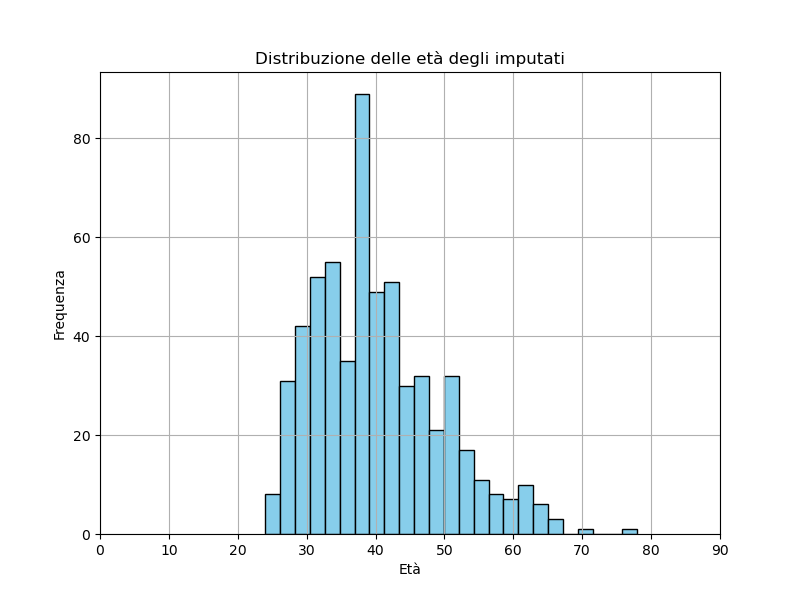
\includegraphics[width= 1 \linewidth]{grafico_eta_media.png}
        \caption{\textit{Età media degli imputati al momento della morte}}
        \label{fig:età_media}
    \end{figure}
  
    \item \textbf{Anno con maggiori/minori esecuzioni}, insieme alla \textbf{media di esecuzioni in un anno}, fornisce una panoramica dell’andamento temporale delle esecuzioni dal 1982 al 2024. La media annuale è di 14 esecuzioni. Come illustrato nella Figura~\ref{fig:esecuzioni_anno}, il 1982 registra il numero minimo di esecuzioni, con una sola condanna portata a termine, mentre il 2000 si distingue come l’anno con il numero massimo, pari a 40 esecuzioni.
    \begin{figure}
        \centering
        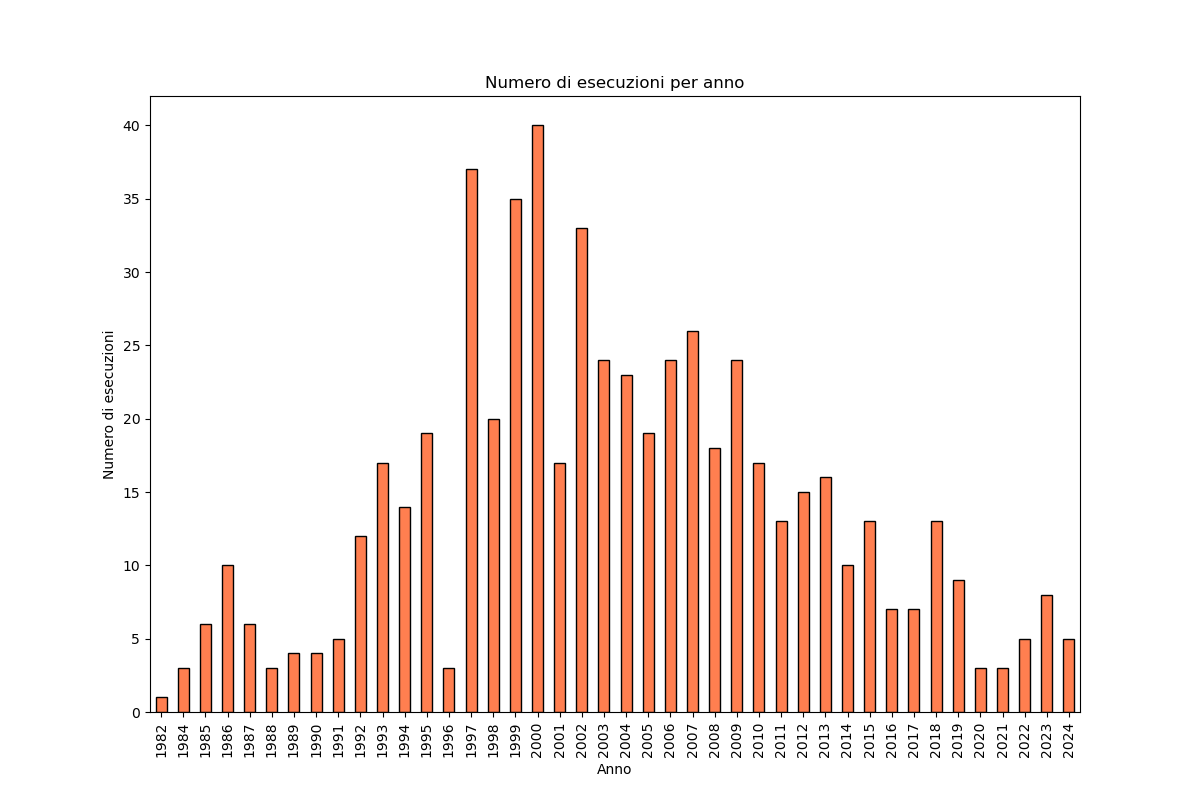
\includegraphics[width=1\linewidth]{grafico_esecuzioni_anno.png}
        \caption{\textit{N° di esecuzioni per anno}}
        \label{fig:esecuzioni_anno}
    \end{figure}
    
    \item \textbf{Distribuzione di frequenza delle etnie tra i condannati a morte}: l’etnia più rappresentata nel dataset è \textit{“White”}, con 263 casi, seguita da \textit{“Black”} (211), \textit{“Hispanic”} (113) e \textit{“Other”} (4). La distribuzione è visualizzata nella Figura~\ref{fig:distr_etnie}, che evidenzia chiaramente la predominanza delle prime tre categorie.
\begin{figure}
        \centering
        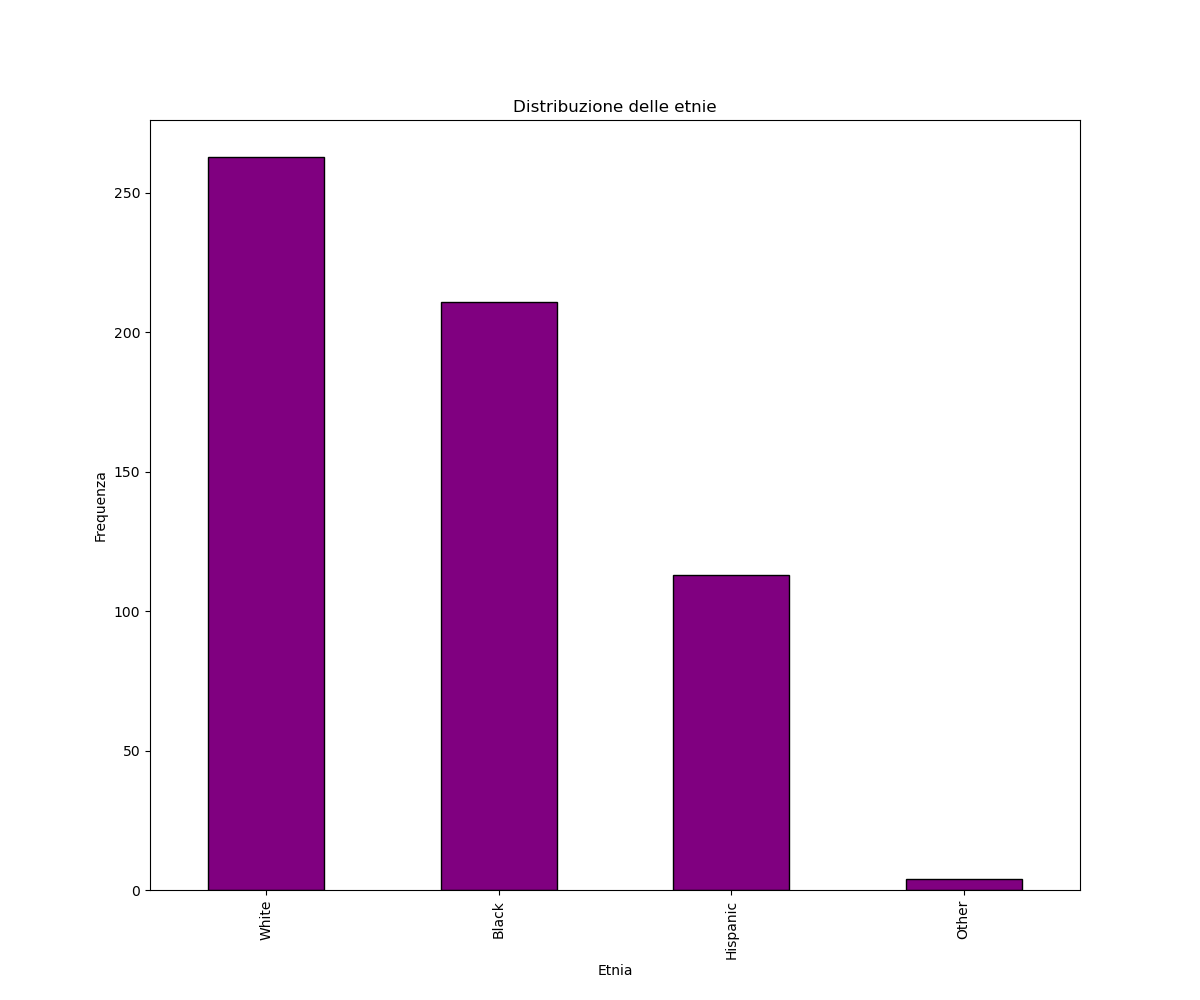
\includegraphics[width=1\linewidth]{grafico_etnie.png}
        \caption{\textit{Distribuzione di frequenza delle etnie}}
        \label{fig:distr_etnie}
    \end{figure}
\\
    \item \textbf{Distribuzione di frequenza dei distretti di appartenenza dei condannati a morte}, analizzata per identificare la loro provenienza. La Figura~\ref{fig:distretti} riporta i primi dieci distretti più rappresentati, con Harris al primo posto con 135 condannati, seguito da Dallas (65), Bexar (46), Tarrant (45) e Nueces (17). Numerosi altri distretti presentano un’unica occorrenza, confermando una concentrazione geografica in specifiche aree del Texas.
    \begin{figure}
        \centering
        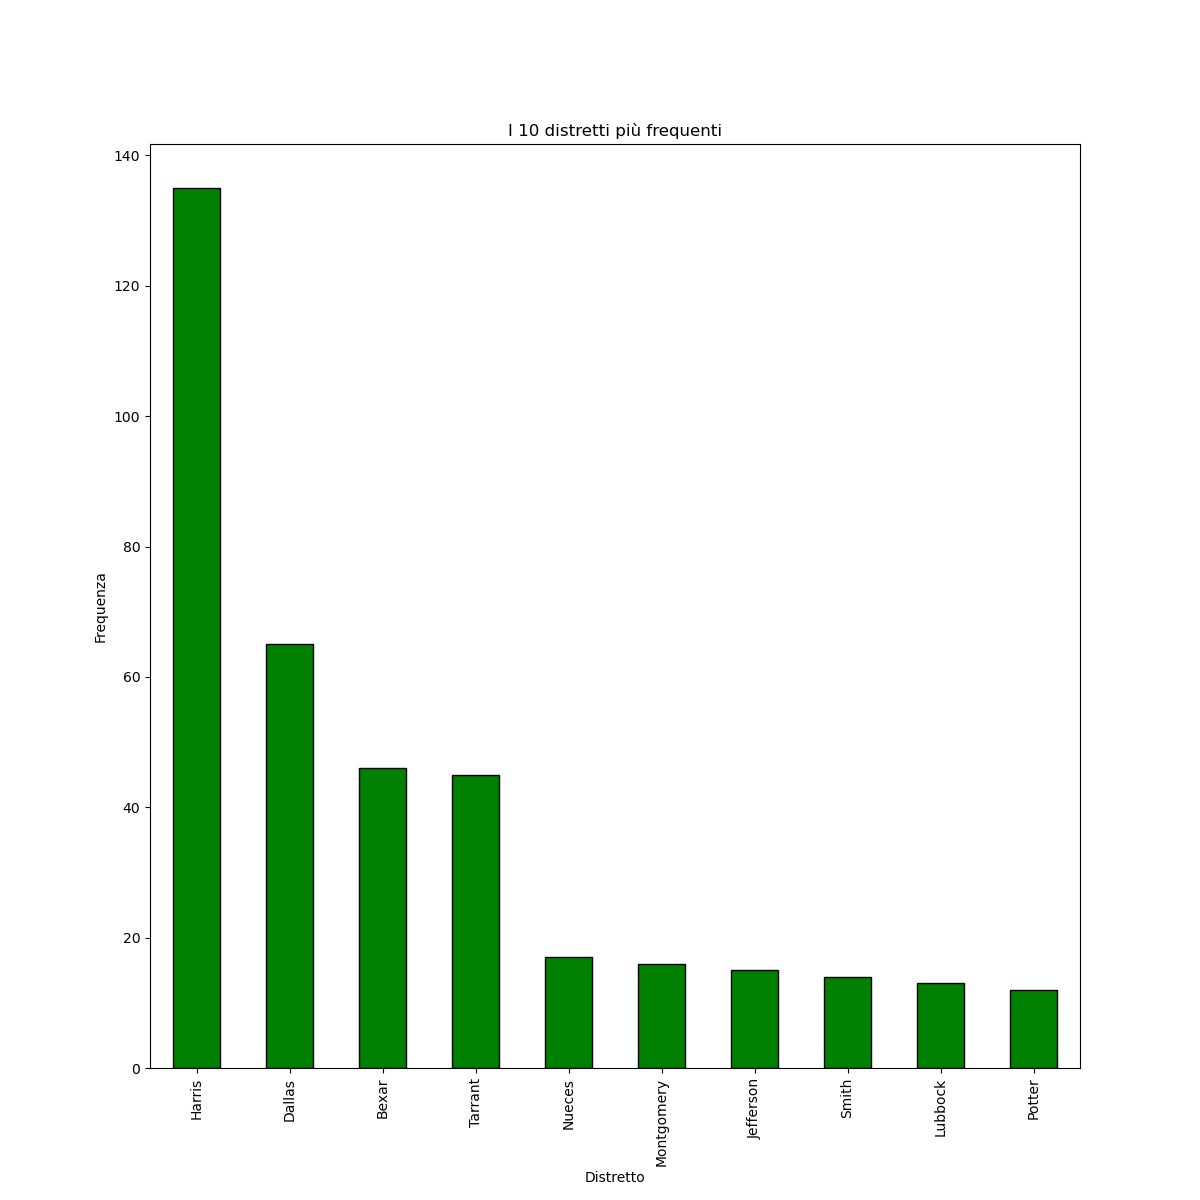
\includegraphics[width=1\linewidth]{grafico_distretti.png}
        \caption{\textit{I 10 distretti più frequenti}}
        \label{fig:distretti}
    \end{figure}
    \item \textbf{Livello di istruzione medio} dei condannati a morte, calcolato sulla base dei dati disponibili. La colonna relativa al “Education Level” presenta alcune anomalie dovute a errori generati dall’utilizzo dell’OCR, come evidenziato nella Figura~\ref{fig:istruzione}. Tuttavia, notiamo che il valore più ricorrente è 12, che corrisponde al \textit{“12th grade”} nel sistema scolastico statunitense, equivalente al quinto anno delle scuole superiori italiane.
    \begin{figure}
        \centering
        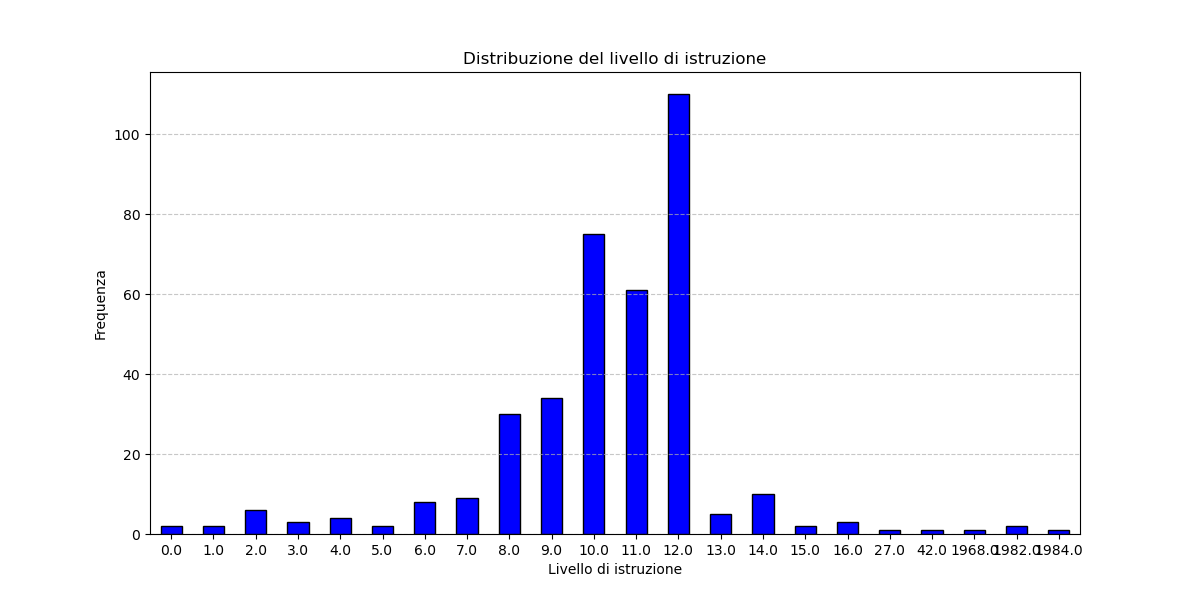
\includegraphics[width=1\linewidth]{grafico_istruzione_bar.png}
        \caption{\textit{Livello di istruzione medio}}
        \label{fig:istruzione}
    \end{figure}
\end{enumerate}

\subsection{Analisi dei dati lessicali}
Questa sezione analizza i dati testuali relativi alle ultime dichiarazioni dei condannati a morte (\textbf{\textit{Last Statement}}) e al riassunto del reato commesso (\textbf{\textit{Summary of Incident}}). Per entrambe le categorie, i testi sono stati sottoposti a un processo di normalizzazione e tokenizzazione, con l’obiettivo di calcolare i token e i bigrammi più frequenti. I risultati ottenuti sono stati rappresentati graficamente e memorizzati in file CSV, contenenti tutti i token e i bigrammi e le relative occorrenze ordinati in ordine decrescente di frequenza.

\begin{itemize}
    \item \textbf{Sezione "\textit{Last Statement}"}
    
    Nell’analisi delle ultime dichiarazioni, abbiamo individuato frasi non rilevanti dal punto di vista lessicale, poiché si trattava di formule standardizzate che indicavano il rifiuto dell’imputato di rilasciare un’ultima dichiarazione. Queste frasi, se incluse, avrebbero potuto distorcere i risultati dell’analisi. Poiché nel dataset non era presente una formulazione unica per tali dichiarazioni, abbiamo effettuato una ricerca per identificare e raccogliere tutte le varianti utilizzate, escludendole successivamente dall’elaborazione dei dati. 
   La Figura~\ref{fig:last_parolefrequenti} mostra le 15 parole più utilizzate nelle ultime dichiarazioni dei condannati a morte. Tra queste, emergono termini fortemente emotivi come \textit{love} (con ben 833 occorrenze si afferma come il più frequente in assoluto), \textit{sorry} e \textit{thank}, che riflettono sentimenti di affetto, rimorso e gratitudine. Parole come \textit{family}, \textit{lord} e \textit{god} evidenziano un legame con i valori della famiglia e della religione, suggerendo che, nei momenti finali, i pensieri dei condannati si rivolgono principalmente a coloro che hanno rappresentato un sostegno emotivo o spirituale durante la loro vita. Questi dati indicano un quadro emotivo complesso, in cui prevalgono messaggi di amore e ringraziamento, ma anche di speranza, accompagnati da riflessioni sul rimorso e sulla fede.
   \begin{figure}
       \centering
       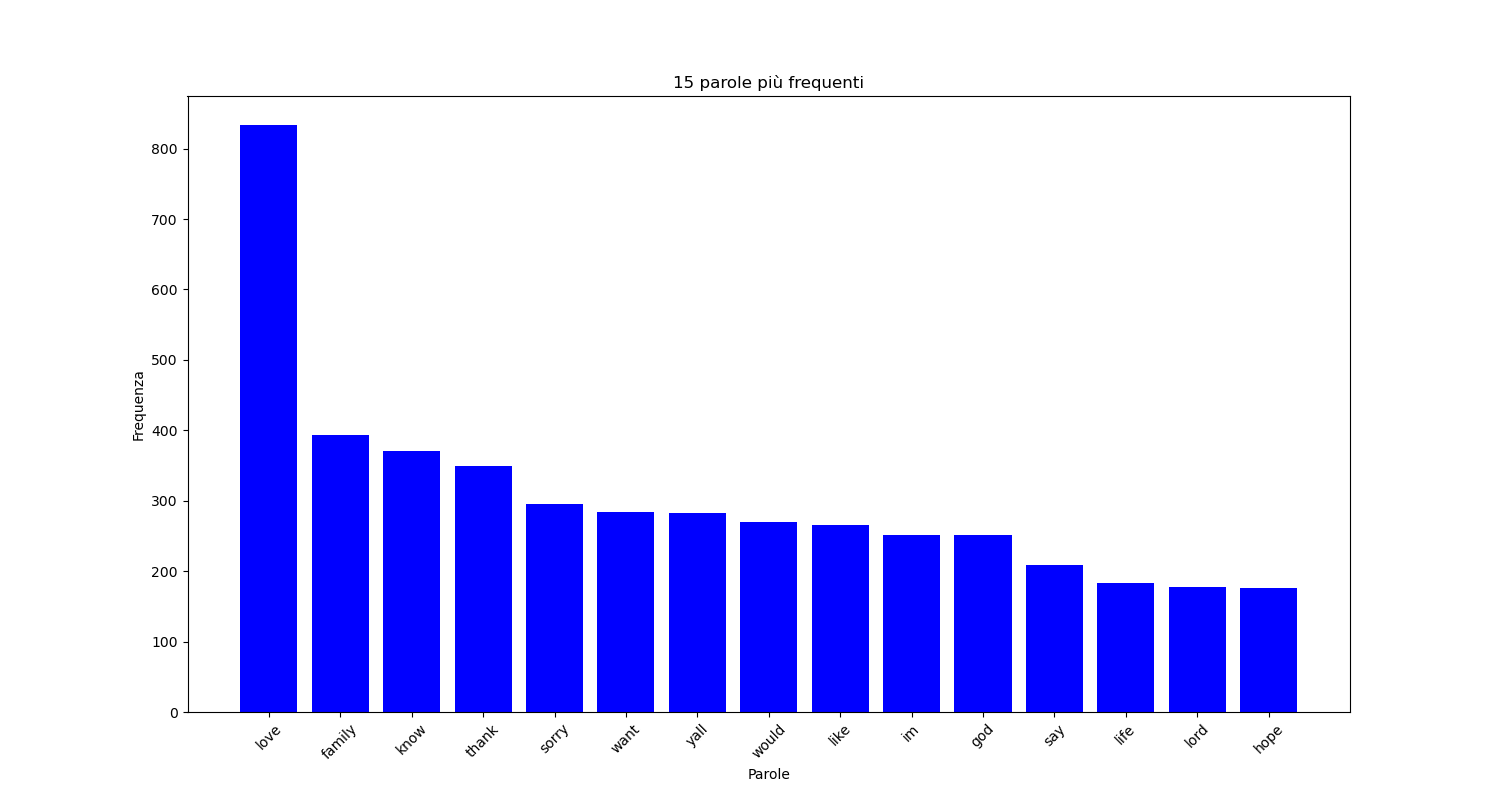
\includegraphics[width=1\linewidth]{last_grafico_parole_frequenti.png}
       \caption{\textit{Le 15 parole più frequenti della sezione "Last Statement}}
       \label{fig:last_parolefrequenti}
   \end{figure}
   \\
   La Figura~\ref{fig:last_bigrammifrequenti} mostra i 10 bigrammi più frequenti nelle ultime dichiarazioni dei condannati a morte. Il bigramma più ricorrente è \textit{would like}, con 175 occorrenze, seguito da espressioni significative come \textit{take care}, \textit{stay strong}, \textit{love family}, dunque messaggi di incoraggiamento rivolti ai familiari e agli amici, mostrando una preoccupazione per i propri cari anche negli ultimi istanti di vita. Tra le espressioni più ricorrenti troviamo anche \textit{im sorry} e \textit{im ready}, che suggeriscono rassegnazione per il destino imminente, ma anche un profondo rimorso per il dolore causato. 
    \begin{figure}
        \centering
        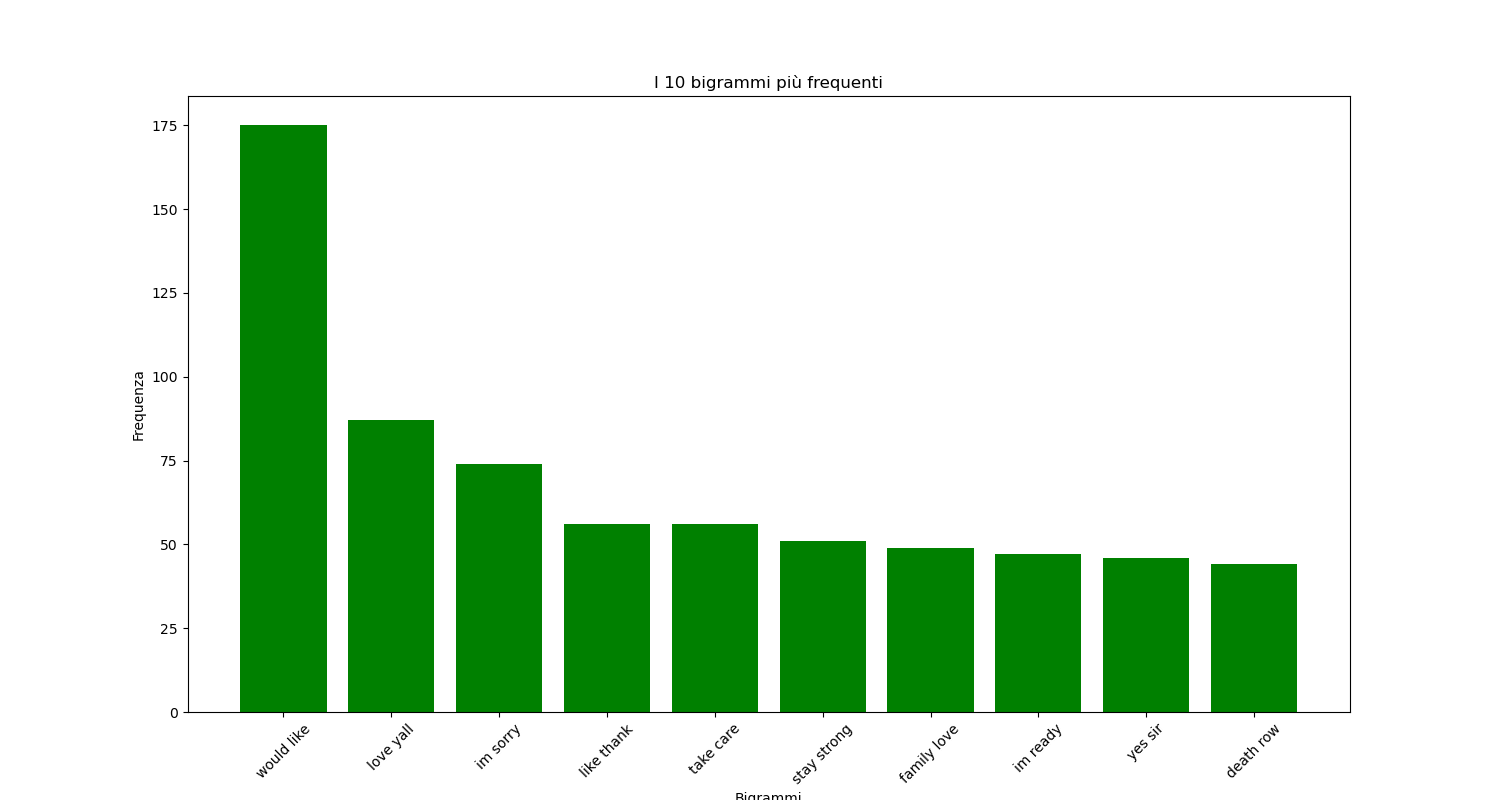
\includegraphics[width=1\linewidth]{last_grafico_bigrammi.png}
        \caption{\textit{I 10 bigrammi più frequenti della sezione "Last Statement"}}
        \label{fig:last_bigrammifrequenti}
    \end{figure}
        \item \textbf{Sezione "\textit{Summary of Incident}"}
       In questa sezione, abbiamo analizzato i riassunti dei reati commessi dai condannati, applicando le stesse tecniche utilizzate nella sezione precedente, ossia la normalizzazione, la tokenizzazione e il calcolo delle frequenze dei termini. La Figura~\ref{fig:summary_parolefrequenti} illustra le 15 parole più frequenti nei riassunti, evidenziando chiaramente la natura dei crimini descritti. Tra i termini più ricorrenti, spiccano quelli legati alla violenza, come \textit{shot} (la parola più frequente con 342 occorrenze), \textit{murder} e \textit{robbery}, nonché quelli che fanno riferimento agli esiti tragici dei crimini, come \textit{death} e \textit{victim}. Inoltre, appaiono parole che indicano i contesti in cui i crimini sono stati commessi o scoperti, come \textit{home}, \textit{car} e \textit{found}. Infine, termini come \textit{police} e \textit{convicted} sottolineano l’aspetto investigativo e giudiziario dei reati descritti.
       \begin{figure}
            \centering
            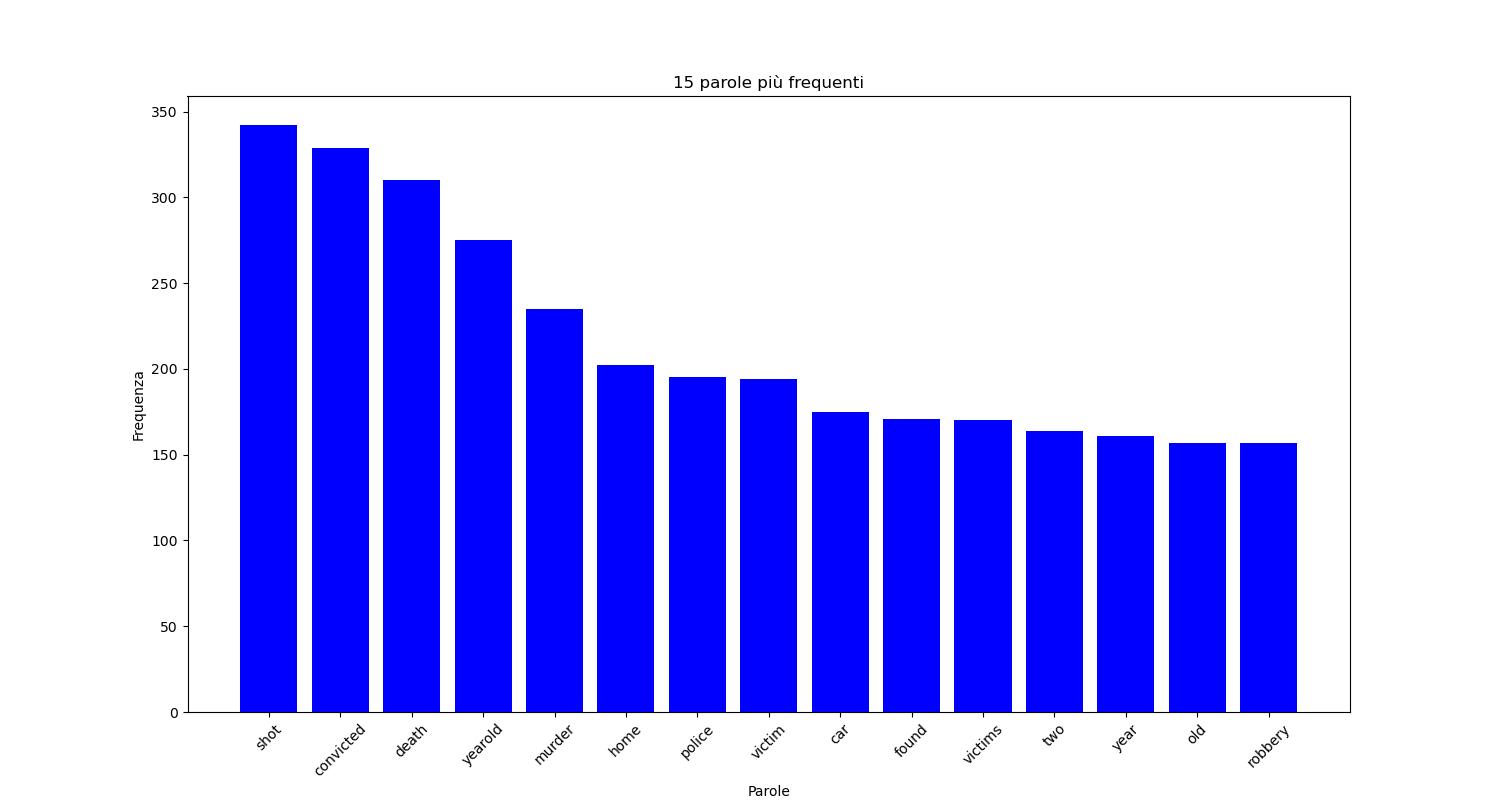
\includegraphics[width=1\linewidth]{summary_grafico_parole_frequenti.png}
            \caption{\textit{Le 15 parole più frequenti della sezione "Summary of Incident"}}
            \label{fig:summary_parolefrequenti}
        \end{figure}

        \begin{figure}
            \centering
            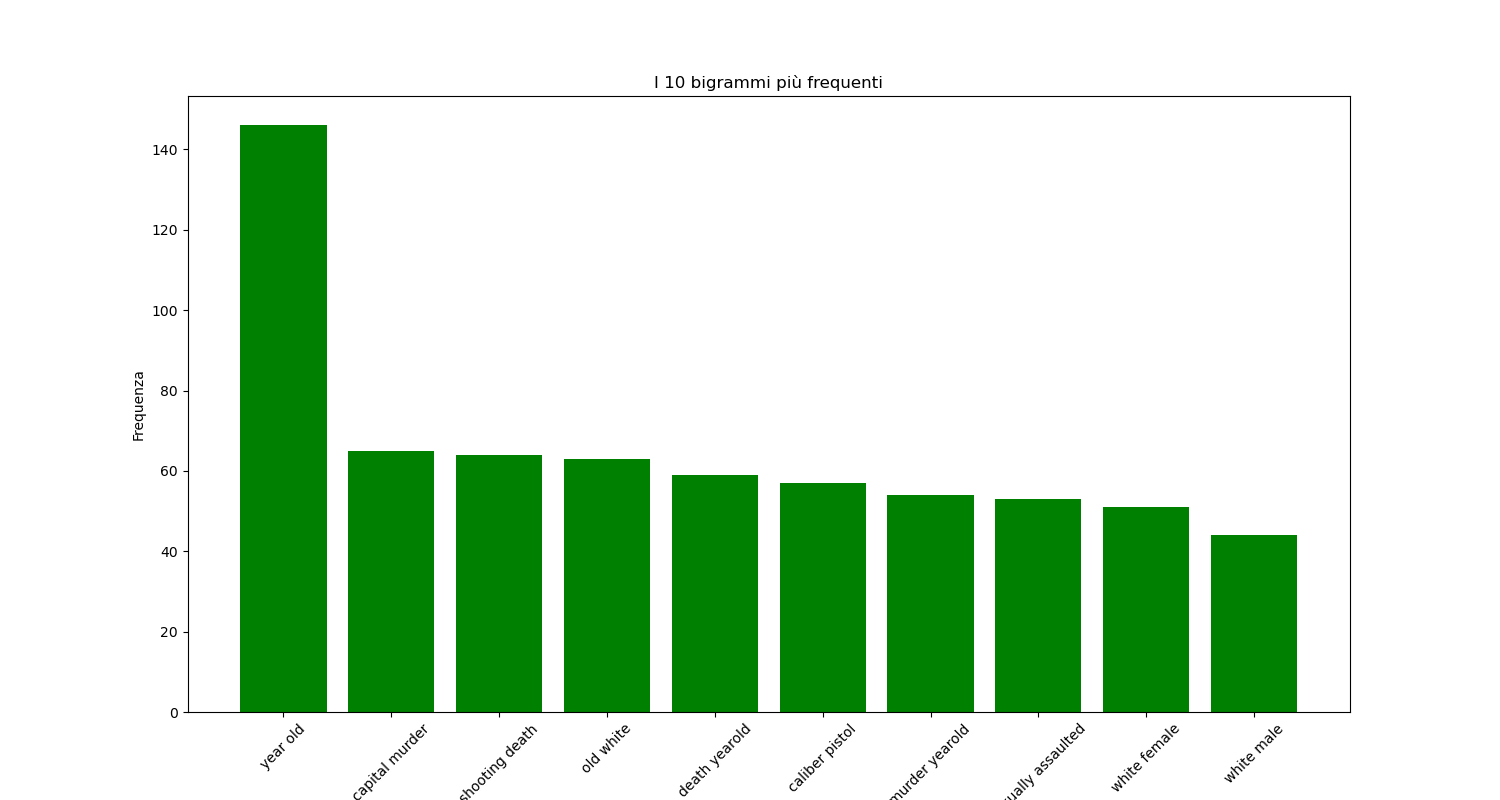
\includegraphics[width=1\linewidth]{summary_grafico_bigrammi.png}
            \caption{\textit{I 10 bigrammi più frequenti della sezione "Summary of Incident"}}
            \label{fig:summary_bigrammifrequenti}
        \end{figure}

        Tra i bigrammi più ricorrenti mostrati nel grafico della Figura~\ref{fig:summary_bigrammifrequenti}, \textit{year old} appare come il più frequente (146 occorrenze), evidenziando l'età delle vittime o dei colpevoli. Un altro bigramma significativo è \textit{capital murder}, che suggerisce l’entità dei crimini commessi, ovvero omicidi capitali, a loro volta seguiti da termini come \textit{shooting death}, \textit{caliber pistol} e \textit{sexually assaulted}, che si riferiscono a modalità e strumenti utilizzati durante l'atto. Questi bigrammi, nel loro complesso, rivelano dettagli chiave sui crimini commessi, sullle caratteristiche delle vittime e sulle modalità con cui sono stati perpetrati.
        
        Tuttavia, ci teniamo a sottolineare che anche in questa sezione è stato utilizzato un OCR per estrarre i dati, il quale ha introdotto del rumore, con la conseguente possibilità che i risultati ottenuti non siano completamente accurati. 
      
\end{itemize}

\section{Fase 4: Valutazione finale}
Per valutare in modo significativo i risultati ottenuti, abbiamo annotato manualmente un campione casuale del dataset, pari al 10\% (59 frasi), con l’obiettivo di creare un Gold Standard per il confronto con le predizioni del modello.
L’annotazione delle emozioni nel Gold Standard è stata effettuata assegnando fino a tre emozioni per ciascuna dichiarazione, selezionando quelle ritenute più rappresentative.
Le prestazioni del modello sono state misurate utilizzando due metriche principali: la percentuale di corrispondenza tra emozioni predette e quelle annotate (\textit{Emotion Match}) e il tasso di correttezza nel riconoscimento del \textit{plea status} (\textit{Correct Plea}). I risultati di queste analisi sono stati inclusi in una colonna aggiuntiva del file CSV.
Dall’analisi emerge che il tasso di corrispondenza tra le emozioni predette e quelle del Gold Standard è pari al \textbf{68,64\%}, mentre la percentuale di correttezza nel riconoscimento del \textit{plea status} raggiunge l’\textbf{81,36\%}.
Tra le emozioni predette e quelle annotate nel Gold Standard, “\textit{love}” risulta essere la più frequente in entrambi i casi. Tuttavia, si osservano alcune differenze nella distribuzione delle emozioni più comuni, come evidenziato nelle tabelle sottostanti.

\begin{table}[H]
\centering
\begin{tabular}{|l|c|}
\hline
\textbf{Predicted Emotion} & \textbf{Frequency} \\ \hline
love           & 28 \\ \hline
hope           & 26 \\ \hline
remorse        & 20 \\ \hline
gratitude      & 20 \\ \hline
acceptance     & 13 \\ \hline
forgiveness    & 12 \\ \hline
regret         & 11 \\ \hline
silence        & 10 \\ \hline
defiance        & 6  \\ \hline
anger           & 5  \\ \hline
\end{tabular}
\caption{10 emozioni più frequenti predette dal modello}
\label{tab:predicted_emotions}
\end{table}

\begin{table}[H]
\centering
\begin{tabular}{|l|c|}
\hline
\textbf{Gold Emotion} & \textbf{Frequency} \\ \hline
love              & 26 \\ \hline
gratitude         & 17 \\ \hline
hope              & 16 \\ \hline
remorse           & 13 \\ \hline
regret             & 8 \\ \hline
forgiveness        & 7 \\ \hline
anger              & 5 \\ \hline
defiance           & 4 \\ \hline
resignation        & 3 \\ \hline
disappointment     & 3 \\ \hline
\end{tabular}
\caption{10 emozioni più frequenti nel Gold Standard.}
\label{tab:gold_emotions}
\end{table}

Per quanto riguarda il riconoscimento del plea status, i risultati sono abbastanza simili a quelli del Gold Standard: notiamo comunque una certa difficoltà nel riconoscere “\textit{guilty}” e “\textit{not guilty}”, con un numero inferiore di predizioni rispetto al Gold Standard come mostra la tabella sottostante. 
\begin{table}[h!]
\centering
\begin{tabular}{|l|c|c|}
\hline
\textbf{Plea Status} & \textbf{Predicted} & \textbf{Gold Standard} \\ \hline
unspecified          & 51                 & 40                     \\ \hline
guilty               & 6                  & 15                     \\ \hline
not guilty           & 2                  & 4                      \\ \hline
\end{tabular}
\caption{Confronto tra il Plea Status Predetto e il Gold Standard}
\label{tab:plea_status}
\end{table}

\section{Conclusioni}
Questo progetto ha rappresentato un’importante esperienza di apprendimento, sia dal punto di vista tecnico che umano. Ha dimostrato l’applicabilità di tecniche avanzate come il web scraping, l’OCR e l’analisi del linguaggio naturale per estrarre e analizzare informazioni da un ampio dataset riguardante i condannati a morte in Texas. 

Nonostante alcune difficoltà, in particolare con l’OCR nell’estrazione del testo dalle immagini, il progetto ha portato alla creazione di un dataset completo e ben strutturato. La valutazione finale del modello, confrontata con un campione annotato manualmente, ha evidenziato risultati promettenti in termini di accuratezza nel riconoscimento delle emozioni e dello stato di colpa. Tuttavia, esistono margini di miglioramento, ad esempio mediante l’uso di modelli alternativi o l’ottimizzazione dei prompt per l’estrazione dei dati. Sebbene il percorso sia ancora lungo, siamo certi che questo rappresenta un buon punto di partenza.





\begin{thebibliography}{}

\bibitem{beautifulsoup}
Beautiful Soup documentation, \url{https://www.crummy.com/software/BeautifulSoup/bs4/doc}

\bibitem{requests}
Requests documentation, \url{https://docs.python-requests.org/en/v2.0.0/}

\bibitem{matplotlib}
Matplotlib documentation, \url{https://matplotlib.org/stable/users/index.html}

\bibitem{numpy}
Numpy documentation, 
\url{https://numpy.org/doc/}

\bibitem{easyocr}
easyOCR documentation, \url{https://www.jaided.ai/easyocr/documentation/}

\bibitem{OpenAI API}
OpenAI API documentation, \url{https://platform.openai.com/docs/api-reference/authentication}

\bibitem{pandas}
Pandas documentation, \url{https://pandas.pydata.org/docs/}

\end{thebibliography}

\end{document}